% chapter3_4.tex -- de (German)
% manual installation of the Phoniebox software
\newpage
\section{Manuelle Installation der \Bezeichnung-Software}

\begin{bclogo}[logo = \bclampe, noborder = true]{Hinweis}
Eigentlich sollte die Installation mit Hilfe des sogenannten
\software{one line installers} funktionieren. Mit etwas Gl�ck l�uft die
Installation problemlos durch, weil alle gemeldeten Fehler durch die
Projekt-Maintainer ausgemerzt wurden. Insbesondere Neulinge sollten
zuerst den \software{one line installer} ausprobieren, bevor sie sich an
den folgenden Einzelkommandos austoben \smiley{wink}\\
\begin{smaller}
\url{https://github.com/MiczFlor/RPi-Jukebox-RFID/wiki/INSTALL-stretch#one-line-install-command}
\end{smaller}
Bei Erfolg kann dieses Kapitel ggf. komplett �bersprungen werden.
\smiley{smile}
\end{bclogo}

Beim {\autor} lief es nat�rlich anders und er f�hrte dann unter 
\os{Raspbian Buster Lite} Anfang Januar 2020 die Installation der
\Bezeichnung-Soft\-ware manuell durch. Dabei traten diverse Probleme
auf, die bei den einzelnen Schritten beschrieben werden. Es kann
nat�rlich jederzeit sein, dass aufgrund von Aktualisierungen im
github-Re\-po\-si\-to\-ry sowohl der \software{one line installer} als
auch die Einzelkommandos wieder funktionieren\dots

Dieses Kapitel orientiert sich dabei an der Installationsanleitung auf
github ab dem Abschnitt \textit{install required packages and the
Phoniebox code}:\\
\begin{scriptsize}
\url{https://github.com/MiczFlor/RPi-Jukebox-RFID/wiki/INSTALL-stretch#install-required-packages-and-the-phoniebox-code}
\end{scriptsize}


\subsection{ben�tigte Programmpakete und -bibliotheken installieren}
\label{sect:apt-get}
F�r den Betrieb der \Bezeichnung-Soft\-ware sind etliche Programmpakete
erforderlich, die �ber \cmd{apt-get} installiert werden. Vor der
Installation empfiehlt es sich, zun�chst das Kommandopaar\\
\cmdPi{sudo apt-get update \&\& sudo apt-get upgrade}\\
abzusetzen, da sich gerade bei \os{Raspbian} in den Repositorys st�ndig
viel �ndert!

\cmdPi{sudo apt-get install apt-transport-https}\\
\cmdPi{sudo apt-get install samba samba-common-bin}
\comment{siehe Abfrage aus Abbildung \ref{fig:apt-get_samba}}\\
\cmdPi{sudo apt-get install python-dev python-pip}\\
\cmdPi{sudo apt-get install \textcolor{red}{python3-dev python3-pip}}
%\comment{Python3 kann hier auf keinen Fall schaden!}\\
\comment{Python3 ist hier kein Fehler!}\\
\cmdPi{sudo apt-get install gcc raspberrypi-kernel-headers lighttpd}\\
\cmdPi{sudo apt-get install php7.3-common php7.3-cgi php7.3 php7.3-fpm}\\
\cmdPi{sudo apt-get install at mpd mpc mpg123}\\
\cmdPi{sudo apt-get install git ffmpeg python-mutagen}\\
\cmdPi{sudo apt-get install \textcolor{red}{python3-mutagen}}
\comment{Python3 schadet auch hier auf keinen Fall!}

\begin{bclogo}[logo = \bclampe, noborder = true]{Hinweis}
In Kapitel \ref{sect:systemd} hat mich dann auch das Fehlen von Python3
eingeholt, weil in der Originalanleitung in Abschnitt \ref{sect:evdev}
nur die Python2-Version installiert wurde\dots \smiley{sarcastic}
\end{bclogo}

\begin{figure}[h]
\centering
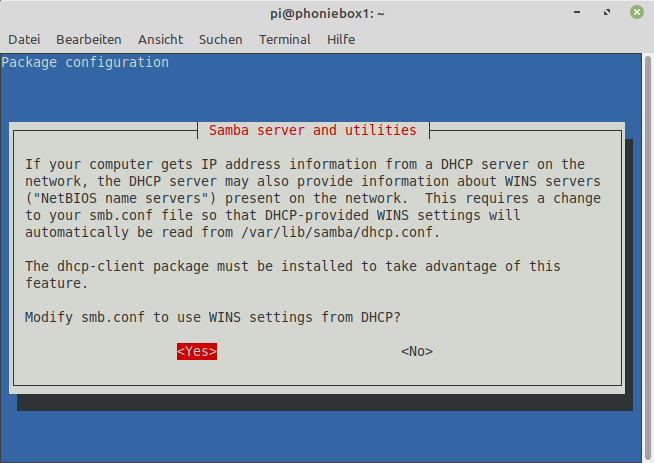
\includegraphics[width=0.88\textwidth, angle=0]{software/apt-get_samba.png}
\caption{Abfrage bei der Installation von \software{Samba} mit \cmd{apt-get}}
\label{fig:apt-get_samba}
\end{figure}

Bei der Installation von \software{Samba} erscheint die Abfrage aus
Abbildung \ref{fig:apt-get_samba}, die wie abgebildet mit \cmd{Yes}
beantwortet wird.
        

\subsection{Projekt \texttt{RPi-Jukebox-RFID} von \textit{github} klonen und installieren}
\cmdPi{git clone https://github.com/MiczFlor/RPi-Jukebox-RFID.git}\\
\cmdPi{cd RPi-Jukebox-RFID}

In der Datei requirements.txt ist (vermutlich au einem alten Stand
herr�hrend) das Paket spidev auskommentiert.

\cmdPi{nano requirements.txt}\\
\editor{\# Library dependencies for the python code.  You need to install these with\\
        \# `sudo pip install -r requirements.txt` before you can run this.\\
        \\
        \#\#\#\# ESSENTIAL LIBRARIES FOR MAIN FUNCTIONALITY \#\#\#\#\\
        \# related libraries.\\
        evdev==0.7.0\\
        git+git://github.com/lthiery/SPI-Py.git\#egg=spi-py\\
        youtube\_dl\\
        pyserial\\
%        \sout{\# spidev - currently installed via apt-get}\comment{eben nicht!}\\
%        \textcolor{blue}{\# added by schlizb�da:\\ spidev}\\
        \textcolor{red}{\# spidev - currently installed via apt-get}\comment{eben nicht!}\\
        RPi.GPIO\\
        pi-rc522
       }
       
\begin{bclogo}[arrondi = 0.2, logo = \bcinfo, ombre = true, epOmbre = 0.25, couleurOmbre = black!30,blur]{Achtung}
Im Gegensatz zum Kommentar in der roten Zeile wird das Paket
\software{spidev} nicht\\installiert. Dies f�hrt zu folgender
Fehlermeldung beim Kommando:\\
\cmdPi{pip install -r requirements.txt}
\end{bclogo}

\begin{smaller}
\begin{verbatim}
Looking in indexes: https://pypi.org/simple, https://www.piwheels.org/simple
Collecting evdev==0.7.0 (from -r requirements.txt (line 7))
  Downloading https://files.pythonhosted.org/packages/67/15/eac376f3e1fc1960a54439c21459b2582e68340001aff83b4ace9e5bd110/evdev-0.7.0.tar.gz
Collecting spi-py from git+git://github.com/lthiery/SPI-Py.git#egg=spi-py (from -r requirements.txt (line 8))
  Cloning git://github.com/lthiery/SPI-Py.git to /tmp/pip-install-uDNQOf/spi-py
Collecting youtube_dl (from -r requirements.txt (line 9))
  Downloading https://files.pythonhosted.org/packages/d0/b3/c3d42f6bbf91da104c272950d30923c222061d7323aa43dcf975a6e8e2c2/youtube_dl-2020.3.24-py2.py3-none-any.whl (1.8MB)
    100% |xxxxxxxxxxxxxxxxxxxxxxxxxxxxxxxx| 1.8MB 129kB/s 
Collecting pyserial (from -r requirements.txt (line 10))
  Downloading https://files.pythonhosted.org/packages/0d/e4/2a744dd9e3be04a0c0907414e2a01a7c88bb3915cbe3c8cc06e209f59c30/pyserial-3.4-py2.py3-none-any.whl (193kB)
    100% |xxxxxxxxxxxxxxxxxxxxxxxxxxxxxxxx| 194kB 608kB/s 
Requirement already satisfied: RPi.GPIO in /usr/lib/python2.7/dist-packages (from -r requirements.txt (line 12)) (0.7.0)
Collecting pi-rc522 (from -r requirements.txt (line 13))
  Downloading https://files.pythonhosted.org/packages/84/f2/e3d02257949e9caa9bff26044e0185e743ff45d3e0e099a93880e10bf718/pi-rc522-2.2.1.tar.gz
    Complete output from command python setup.py egg_info:
    Traceback (most recent call last):
      File "<string>", line 1, in <module>
      File "/tmp/pip-install-uDNQOf/pi-rc522/setup.py", line 11, in <module>
        from pirc522 import __version__  # flake8: noqa
      File "pirc522/__init__.py", line 4, in <module>
        from .rfid import RFID
      File "pirc522/rfid.py", line 2, in <module>
        import spidev
    ImportError: No module named spidev
\end{verbatim}
\textcolor{red}{Command "python setup.py egg\_info"\ failed with error code 1 in /tmp/pip-install-uDNQOf/pi-rc522/}
\end{smaller}

\textbf{Deshalb die Python-Software so installieren:}\\
\cmdPi{echo spidev >spidev.txt}\\
\cmdPi{pip install -r spidev.txt}\\
\cmdPi{pip install -r requirements.txt}

Hiermit l�uft die Python-Installation fehlerfrei durch!


\subsection{Einbinden des RFID-Lesers als Python(?)-Event}
\label{sect:evdev}
\cmdPi{pip install evdev}
\begin{smaller}
\begin{verbatim}
Looking in indexes: https://pypi.org/simple, https://www.piwheels.org/simple
Requirement already satisfied: evdev in /home/pi/.local/lib/python2.7/site-packages (0.7.0)
\end{verbatim}
\end{smaller}

\begin{bclogo}[logo = \bclampe, noborder = true]{Hinweis}
Aufgrund der obigen Meldung scheint das Python2-Paket \texttt{evdev}
bereits aktuell zu sein. \textcolor{red}{Viel wichtiger ist aber, dass
diese Bibliothek anschlie�end auch f�r \software{Python3} installiert
wird!}
\end{bclogo}

\cmdPi{pip3 install evdev}
\begin{smaller}
\begin{verbatim}
Looking in indexes: https://pypi.org/simple, https://www.piwheels.org/simple
Collecting evdev
  Downloading https://www.piwheels.org/simple/evdev/evdev-1.3.0-cp37-cp37m-linux_armv7l.whl (98kB)
    100% |xxxxxxxxxxxxxxxxxxxxxxxxxxxxxxxx| 102kB 628kB/s 
Installing collected packages: evdev
Successfully installed evdev-1.3.0
\end{verbatim}
\end{smaller}


\subsection{Webserver \software{lighttpd} f�r die Web-App der {\Bezeichnung} einrichten}
Auch bei der Web-App l�uft's ganz und gar nicht wie geschmiert.
\smiley{nosmile}

\textbf{Datei \filenam{/etc/lighttpd/lighttpd.conf} bearbeiten}\\
In der Datei \filenam{/etc/lighttpd/lighttpd.conf} m�ssen folgende
�nderungen (rot) erg�nzt werden:\\
\cmdPi{sudo nano /etc/lighttpd/lighttpd.conf}\\
\editor{\textcolor{red}{\# adjusted by schlizb�da due to https://github.com/MiczFlor/RPi-Jukebox-RFID/wiki/INSTALL-stretch\#lighttpd-web-server-for-web-app\\
server.document-root        = "/home/pi/RPi-Jukebox-RFID/htdocs"\\
\#}server.document-root        = "/var/www/html"\\
server.upload-dirs          = ( "/var/cache/lighttpd/uploads" )\\
server.errorlog             = "/var/log/lighttpd/error.log"\\
server.pid-file             = "/var/run/lighttpd.pid"\\
server.username             = "www-data"\\
server.groupname            = "www-data"\\
server.port                 = 80
}

\textbf{Datei \filenam{/etc/sudoers} bearbeiten}\\
Hier muss hinten der rot eingef�rbte Teil angeh�ngt werden:\\
\editor{\#\\
\# This file MUST be edited with the 'visudo' command as root.\\
\#\\
\# Please consider adding local content in /etc/sudoers.d/ instead of\\
\# directly modifying this file.\\
\#\\
\# See the man page for details on how to write a sudoers file.\\
\#\\
Defaults        env\_reset\\
Defaults        mail\_badpass\\
Defaults        secure\_path="/usr/local/sbin:/usr/local/bin:/usr/sbin:/usr/bin:/sbin:/bin"
}
%\\
%\# Host alias specification\\
%\\
%\# User alias specification\\
%\\
%\# Cmnd alias specification\\
%\\
%\# User privilege specification\\
%root    ALL=(ALL:ALL) ALL\\
%\\
%\# Allow members of group sudo to execute any command\\
%%sudo   ALL=(ALL:ALL) ALL\\
%\\
%\# See sudoers(5) for more information on "\#include" directives:\\
%\\
%\#includedir /etc/sudoers.d\\
%\\
\texttt{\\
\begin{small}%\textcolor{gray}{\vdots}\\
    \textcolor{red}{\textit{\# added by schlizb�da:\\www-data ALL=(ALL) NOPASSWD: ALL}}
    \\\textcolor{gray}{\vdots}
\end{small}}

\textbf{Modul \texttt{fastcgi} f�r den Webserver \software{lighttpd} konfigurieren}\\
Damit der Webserver die bei der {\Bezeichnung} zum Einsatz kommenden
HP-Scrip\-te ausf�hren kann, muss das Modul \texttt{fastcgi} mit den
folgenden Kommandos einmalig aktiviert werden:\\
\cmdPi{sudo lighttpd-enable-mod fastcgi}\\
\stdout{Enabling fastcgi: ok\\
        Run "{}service lighttpd force-reload"\ to enable changes}\\
\cmdPi{sudo lighttpd-enable-mod fastcgi-php}\\
\stdout{Enabling fastcgi-php: ok\\
        Run "{}service lighttpd force-reload" to enable changes}

%M�glicherweise ist die Konfiguration noch auf PHP5 eingestellt. F�r die
%{\Bezeichnung} wird aber PHP7 ben�tigt. Daher muss die Datei
%\filenam{/etc/lighttpd/conf-available/15-fastcgi-php.conf} angepasst
%werden.
%\begin{bclogo}[arrondi = 0.2, logo = \bcinfo, ombre = true, epOmbre = 0.25, couleurOmbre = black!30,blur]{Achtung}
%Unter \os{Raspbian Buster} kommt mittlerweile \textcolor{red}{PHP7.3}
%zum Einsatz, nicht mehr PHP7.0! Von daher muss beim Editieren auch die
%richtige Versionsnummer eingetragen werden.\\
%Auch dies wurde in der Anleitung unter\\
%\begin{scriptsize}\url{https://github.com/MiczFlor/RPi-Jukebox-RFID/wiki/INSTALL-stretch#lighttpd-web-server-for-web-app}\end{scriptsize}\\
%noch nicht ber�cksichtigt und angepasst!
%\end{bclogo}
%\cmdPi{sudo nano /etc/lighttpd/conf-available/15-fastcgi-php.conf}\\
%\editor{\# -*- depends: fastcgi -*-\\
%\# /usr/share/doc/lighttpd/fastcgi.txt.gz\\
%\# http://redmine.lighttpd.net/projects/lighttpd/wiki/Docs:ConfigurationOptions\#mod\_fastcgi-fastcgi\\
%\\
%\#\# Start an FastCGI server for php (needs the php5-cgi package)\\
%fastcgi.server += ( ".php" =>\\
%\tab[1cm]((\\
%\tab[2cm]"{}socket" => "/var/run/php/\textcolor{red}{php7.3-fpm.sock}",\\
%\tab[2cm]"broken-scriptfilename" => "{}enable"\\
%\tab[1cm]))
%)}

Die neue Konfiguration des \software{lighttpd}-Webservers neu laden:\\
\cmdPi{sudo service lighttpd force-reload}


\textbf{Upload von Audiodateien �ber den Webservice erm�glichen}\\
Um den Webservice f�r den Upload von Audiodateien auf die {\Bezeichnung}
zu ert�chtigen, muss die Datei \filenam{/etc/php/7.3/fpm/php.ini}
angelegt werden. Dazu ist im github-Repository der {\Bezeichnung} eine
Beispieldatei vorhanden:\\
\cmdPi{\begin{scriptsize}sudo cp /home/pi/RPi-Jukebox-RFID/misc/sampleconfigs/php.ini.stretch-default.sample /etc/php/\textcolor{red}{7.3}/fpm/php.ini\end{scriptsize}}
\cmdPi{sudo chown root:root /etc/php/\textcolor{red}{7.3}/fpm/php.ini}\\
\cmdPi{sudo chmod 644 /etc/php/\textcolor{red}{7.3}/fpm/php.ini}

In der Datei \texttt{/etc/php/7.3/fpm/php.ini} sind folgende Eintr�ge zu
kontrollieren und gegebenenfalls zu erg�nzen:\\
\cmdPi{sudo nano /etc/php/\textcolor{red}{7.3}/fpm/php.ini}\\
\editor{file\_uploads = On\\
upload\_max\_filesize = 0\\
max\_file\_uploads = 20\\
post\_max\_size = 0
}

\cmdPi{sudo service \textcolor{red}{php7.3-fpm} restart}


\textbf{Konfigurationsdatei f�r die Web-App aus der Beispieldatei kopieren}\\
\cmdPi{\begin{smaller}cp /home/pi/RPi-Jukebox-RFID/htdocs/config.php.sample /home/pi/RPi-Jukebox-RFID/config.php\end{smaller}}

\textbf{Zugriff auf Verzeichnisse \filenam{shared} und \filenam{htdocs} f�r den Webservice erm�glichen}\\
Der Zugriff erfolgt unter dem Benutzer \texttt{www-data}, daher muss der
Zugriff auf die beiden Verzeichnisse f�r diesen Benutzer �ber
Gruppenrechte erm�glicht werden:\\
\cmdPi{sudo chown -R pi:www-data /home/pi/RPi-Jukebox-RFID/shared}\\
\cmdPi{sudo chmod -R 775 /home/pi/RPi-Jukebox-RFID/shared}\\
\cmdPi{sudo chown -R pi:www-data /home/pi/RPi-Jukebox-RFID/htdocs}\\
\cmdPi{sudo chmod -R 775 /home/pi/RPi-Jukebox-RFID/htdocs}


\newpage
\textbf{Kontrolle im Browser:}\\
\begin{figure}[!h]
\centering
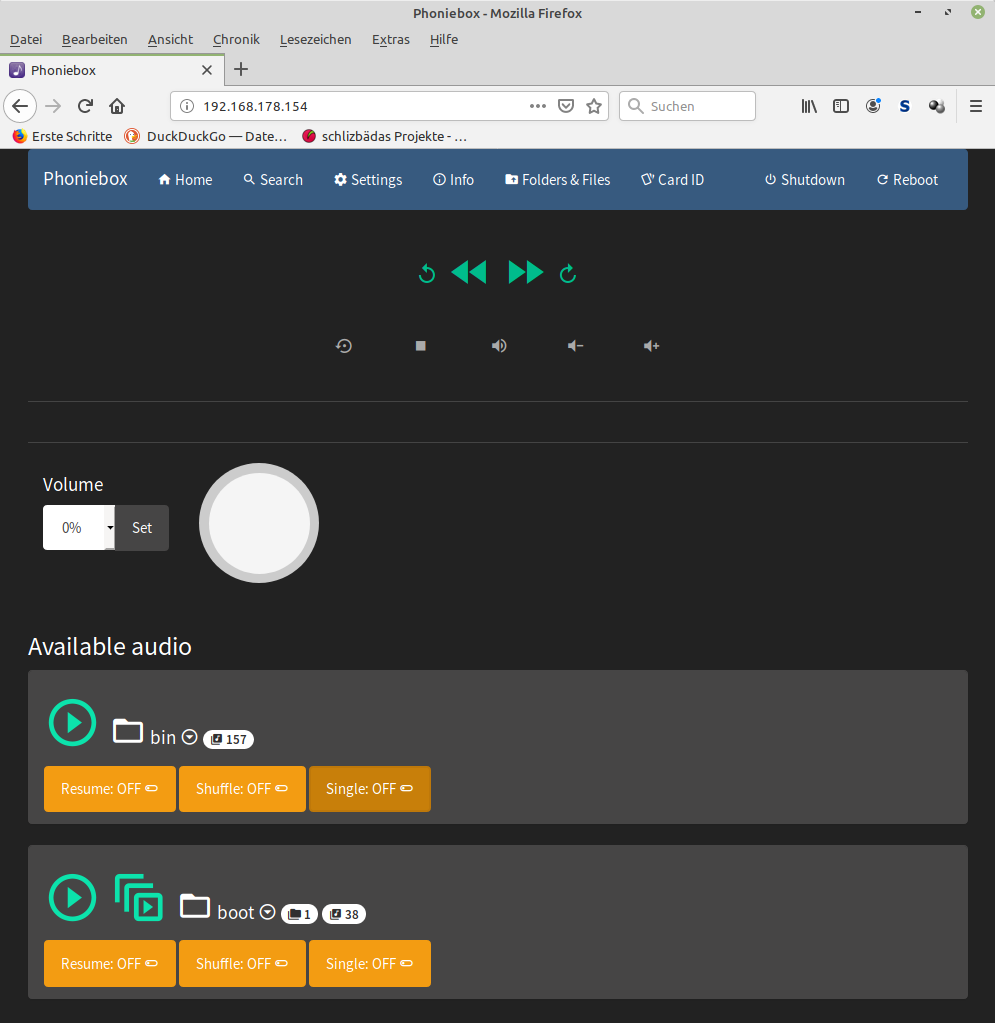
\includegraphics[width=1\textwidth, angle=0]{software/lighttpd_webserver.png}
\caption{Aufruf des \software{lighttpd}-Webservers}
\label{fig:lighttpd_webserver}
\end{figure}

Hintergrunddetails zur Einrichtung des Webservers siehe:\\
\begin{smaller}
\url{https://github.com/MiczFlor/RPi-Jukebox-RFID/wiki/INSTALL-stretch#lighttpd-web-server-for-web-app}
\end{smaller}
